% Created 2023-02-27 Mon 20:19
% Intended LaTeX compiler: pdflatex
\documentclass[presentation,aspectratio=169]{beamer}
\usepackage[utf8]{inputenc}
\usepackage[T1]{fontenc}
\usepackage{graphicx}
\usepackage{grffile}
\usepackage{longtable}
\usepackage{wrapfig}
\usepackage{rotating}
\usepackage[normalem]{ulem}
\usepackage{amsmath}
\usepackage{textcomp}
\usepackage{amssymb}
\usepackage{capt-of}
\usepackage{hyperref}
\usepackage{khpreamble, euscript}
\DeclareMathOperator{\atantwo}{atan2}
\newcommand*{\ctrb}{\EuScript{C}}
\newcommand*{\obsv}{\EuScript{O}}
\usetheme{default}
\author{Kjartan Halvorsen}
\date{\today}
\title{El modelo canónico de robots móviles no-holonómicos}
\hypersetup{
 pdfauthor={Kjartan Halvorsen},
 pdftitle={El modelo canónico de robots móviles no-holonómicos},
 pdfkeywords={},
 pdfsubject={},
 pdfcreator={Emacs 26.3 (Org mode 9.4.6)}, 
 pdflang={English}}
\begin{document}

\maketitle

\section{Mobile robots}
\label{sec:orgfd76dd5}

\begin{frame}[label={sec:org9a51b3d}]{Modelo canónico a.k.a modelo uniciclo}
\begin{center}
 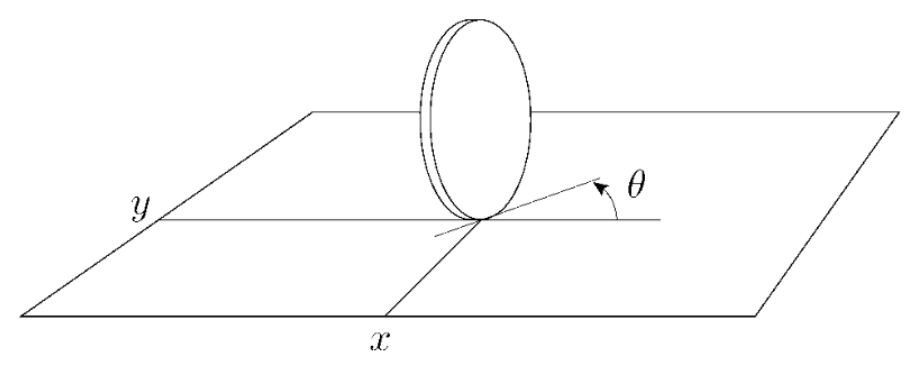
\includegraphics[width=.6\linewidth]{../figures/unicycle-kth.png}
\end{center}

\footnotesize
De Martina Zambelli (2013) \emph{Posture regulation for unicycle-like robots with prescribed performance guarantees}. KTH - Royal Institute of Technology, Sweden.
\end{frame}


\section{Differential drive}
\label{sec:org1d21ebe}

\begin{frame}[label={sec:org163cf4c}]{Robot tipo diferencial (\emph{differential drive})}
\begin{center}
 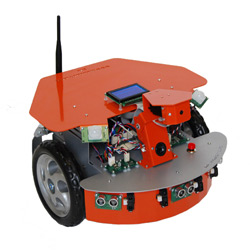
\includegraphics[width=.5\linewidth]{../figures/X80Pro.jpg}
\end{center}

X80Pro Dr. Robot Inc.
\end{frame}

\begin{frame}[label={sec:org9105af5}]{Robot móvil - modelo canónico}
\begin{columns}
\begin{column}{0.4\columnwidth}
\begin{center}
 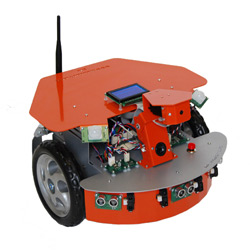
\includegraphics[width=.3\linewidth]{../figures/X80Pro.jpg}
\end{center}
\begin{center}
 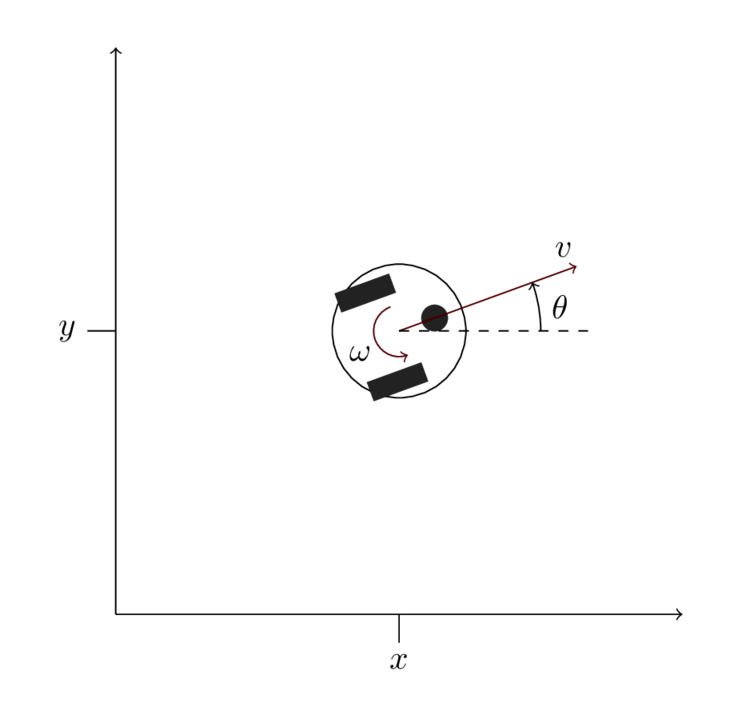
\includegraphics[width=1.0\linewidth]{../figures/unicycle-model}
\end{center}
\end{column}

\begin{column}{0.6\columnwidth}
\pause

\alert{Cinemática}

\[ \xi = \begin{bmatrix} \theta\\x\\y \end{bmatrix},   \quad u = \begin{bmatrix} \omega\\v \end{bmatrix}\]



\[\frac{d}{dt} \xi = \begin{bmatrix} \dot{\theta}\\\dot{x}\\\dot{y} \end{bmatrix} = \begin{bmatrix} \omega\\ v\cos\theta\\v\sin\theta\end{bmatrix} \]


\pause

\alert{Actividad} En simulink
\end{column}
\end{columns}
\end{frame}



\begin{frame}[label={sec:org29a6f2f}]{De robot diferencial a modelo canónico}
\begin{columns}
\begin{column}{0.4\columnwidth}
\begin{center}
 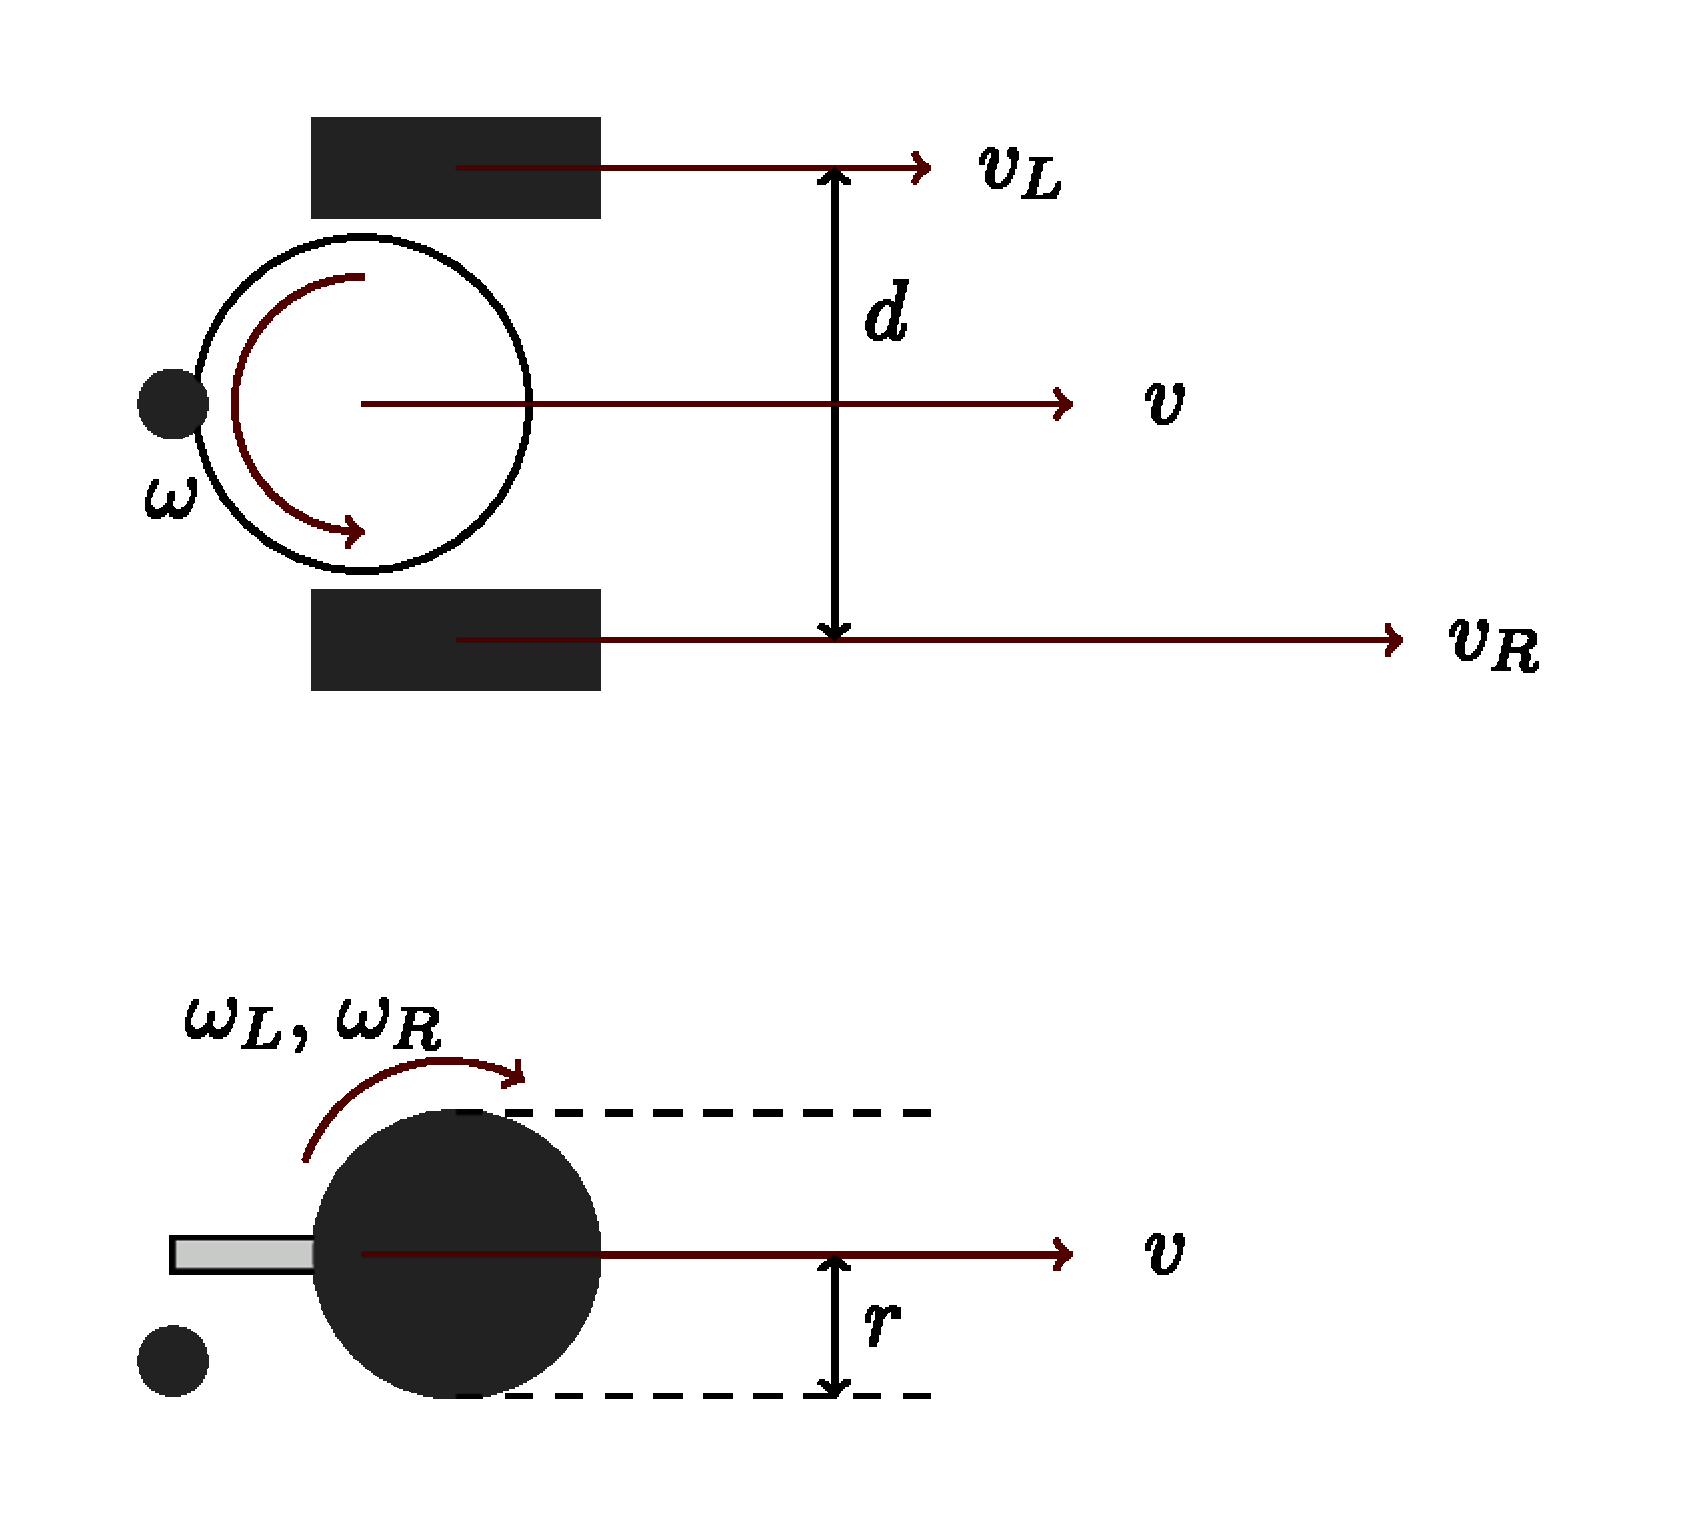
\includegraphics[width=1.0\linewidth]{../figures/unicycle-model-details}
\end{center}
\end{column}

\begin{column}{0.6\columnwidth}
\pause

\alert{Actividad} Determine

\begin{enumerate}
\item La velocidad lineal (\(v_R\), \(v_L\)) del centro de cada rueda dado su velocidad angular (\(\omega_R\), \(\omega_L\))

\item La velocidad lineal \(v\) del centro robot dado las dos velocidades \(v_R\) y \(v_L\)

\item La velocidad angular \(\omega\) del robot dado las dos velocidades \(v_R\) y \(v_L\)
\end{enumerate}


\begin{enumerate}
\item Las relaciones invertidas. Es decir, las velocidades angulares \(\omega_R\) y \(\omega_L\) de las ruedas dado las velocidades \(v\) y \(\omega\).
\end{enumerate}
\end{column}
\end{columns}
\end{frame}

\begin{frame}[label={sec:org330e57c}]{Diferencial a modelo canónico}
\begin{columns}
\begin{column}{0.4\columnwidth}
\begin{center}
 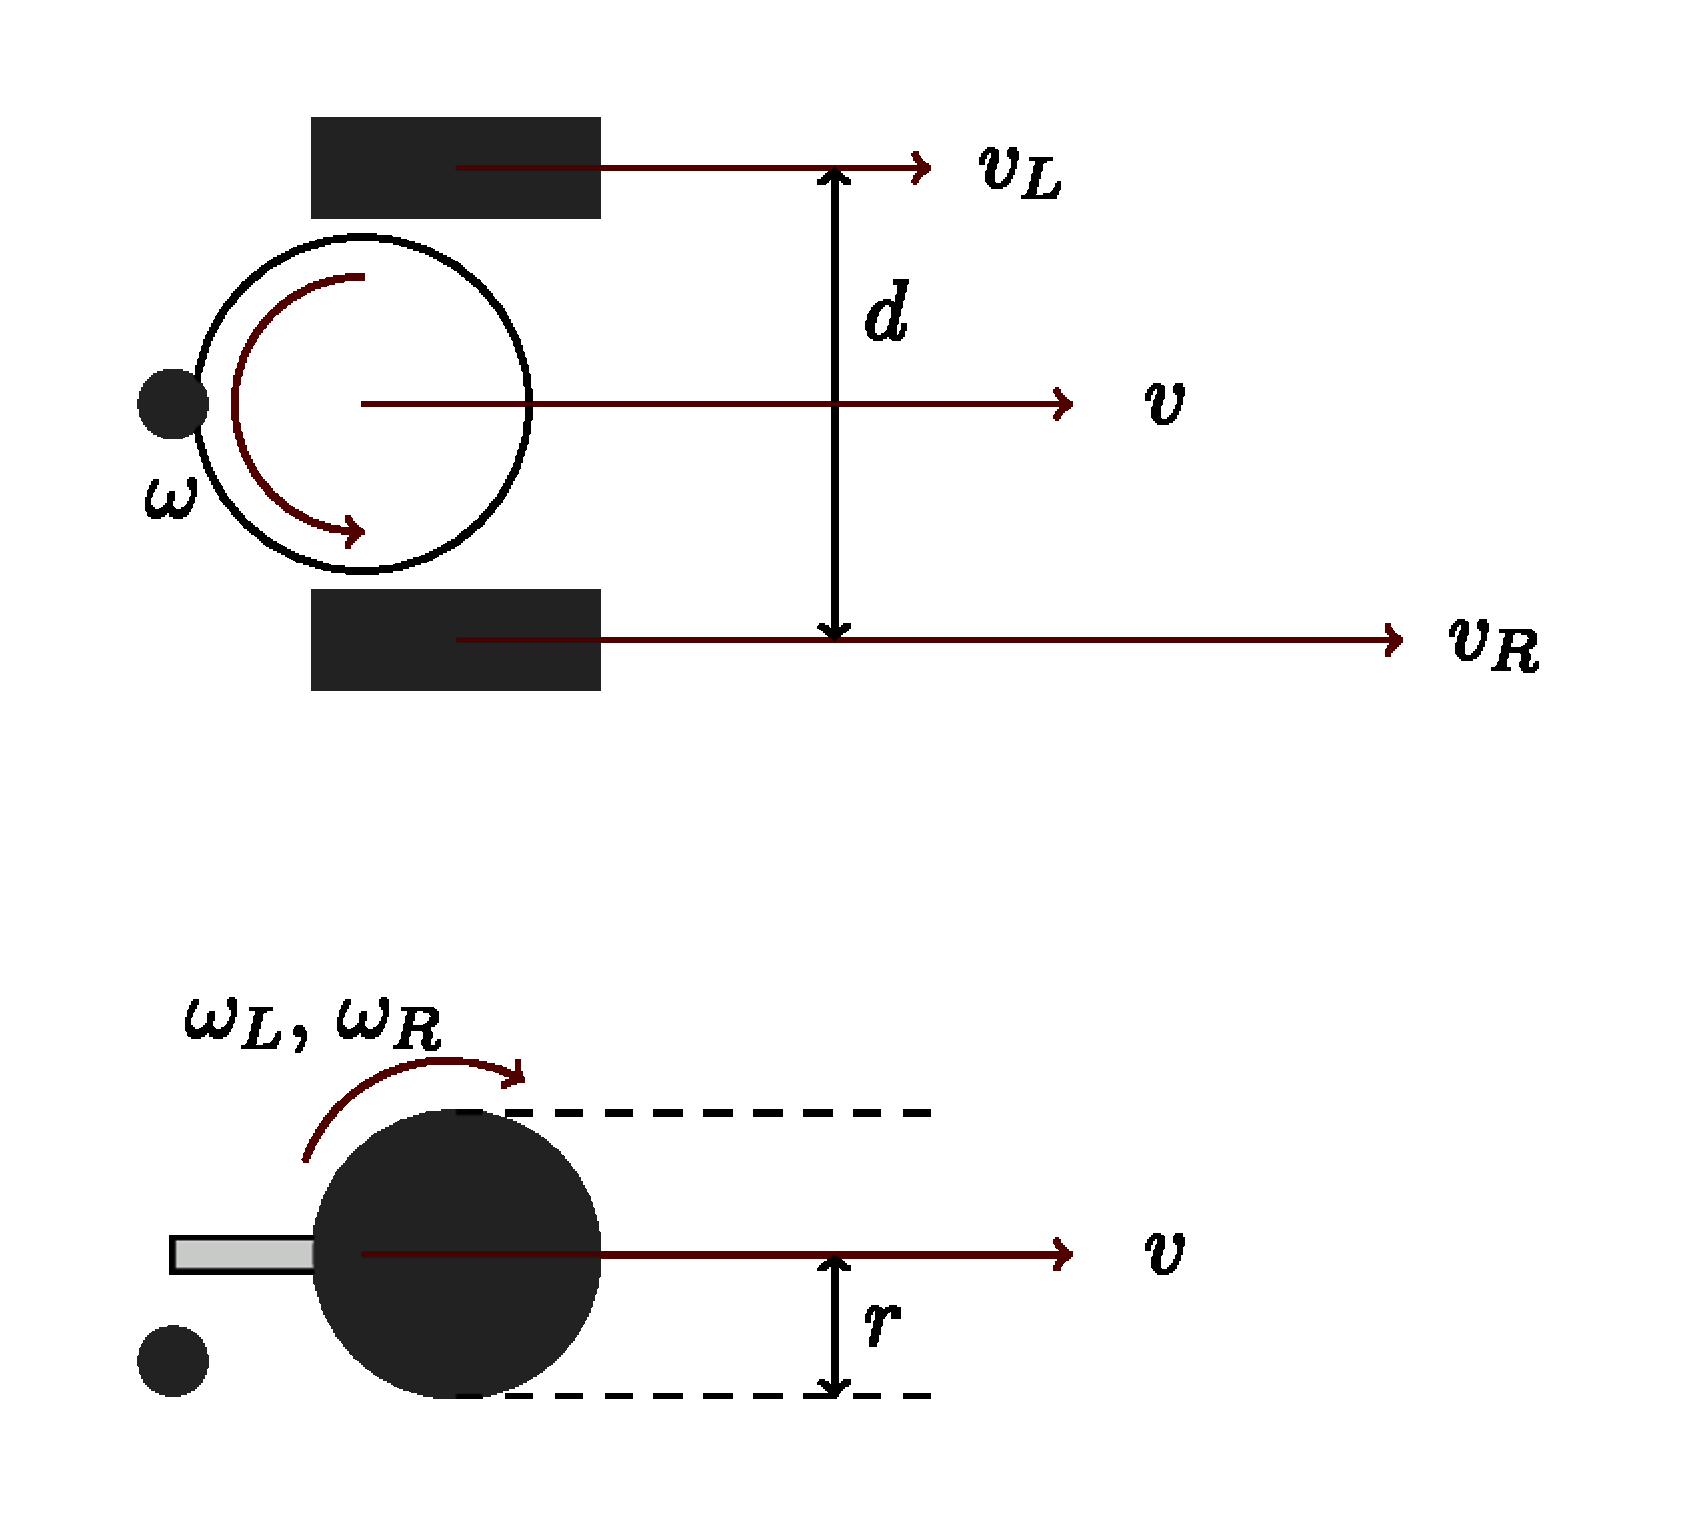
\includegraphics[width=.8\linewidth]{../figures/unicycle-model-details}
\end{center}
\end{column}

\begin{column}{0.6\columnwidth}
Asumiendo simetría entre las dos ruedas y en la dirección de giro.

\[ \omega_L,\, \omega_R \; \in \; [-\omega_{max}, \omega_{max}]\]

\pause

\alert{Actividad}
En el plano \(v,\, \omega\),  dibuje la región de posibles valores de la señal de entrada al modelo canónico,
\[ u(t) = \begin{bmatrix} \omega(t)\\v(t) \end{bmatrix}, \]
dado los límites de la velocidad angular de las ruedas.
\end{column}
\end{columns}
\end{frame}
\end{document}